% !TEX encoding = UTF-8 Unicode
% -*- coding: UTF-8; -*-
\documentclass[10pt]{beamer}

\usepackage[frenchb]{babel}
\usepackage[T1]{fontenc}
\usepackage[utf8]{inputenc}
\usepackage{hyperref}
\usepackage{listings}
\usepackage{fancyvrb}
\usepackage{tikz}
\usepackage{framed}
\usepackage{algorithm}
\usepackage{algorithmic}
  \usepackage{amsmath,amssymb,amsthm}
  \usepackage{dsfont}\let\mathbb\mathds
\usepackage{setspace}
\usepackage{pgfplots}

\usetikzlibrary{shapes.geometric}
\usetikzlibrary{shapes.arrows}
\usetikzlibrary{arrows}
\usepackage{array}

%\usetheme{Boadilla}
\usetheme{inria}
\usepackage{helvet}
\usecolortheme{dolphin}
\newcommand{\R}{\mathbb{R}}
\newcommand{\C}{\mathbb{C}}
\newcommand{\N}{\mathbb{N}}
\newcommand{\Z}{\mathbb{Z}}


\newcommand{\inriaswitchcolors}[1]{%
\pgfaliasimage{figfootline}{figfootline-#1}% !!!
\pgfaliasimage{figbackground}{figbackground-#1}% !!!
\pgfaliasimage{figbackground}{figbackground-#1}% !!!
}

%\inriaswitchcolors{pastelgreen}
\lstnewenvironment{codeC}
{ \lstset{language=C,
    otherkeywords={printf,scan}}
}
{}
\newcommand{\red}{\textcolor{red}}
\newcommand{\plus}[1]{\textcolor{orange}{\textbf{#1}}}
%\newcommand \emph
%Default size : 12.8 cm * 9.6 cm

\newenvironment<>{codeblock}[1]{%begin
  \setbeamercolor{block title}{fg=darkgray,bg=yellow}%
  \begin{block}{#1}}
  % \begin{codeC}}
  %  {\end{codeC}
{  
\end{block}}

\newenvironment<>{termblock}[1]{
    \setbeamercolor{block title}{fg=white,bg=lightgray}%
    \begin{block}{#1}}
%     \begin{Verbatim}}
{%\end{Verbatim}
\end{block}
}
%\newcommand{\output}[1]{

%%% Paramètres du cours (à régler)
%Numéro du cours
\newcommand{\nb}{1}
\setbeamertemplate{navigation symbols}{}%remove navigation symbols

\title[Bilan/perspective]{Délégation à CLIME : \mbox{Bilan/perspective}} %mbox insecable
\subtitle{2014-2016}
\author[J. Brajard]{Julien Brajard}
\institute[CLIME]{Inria CLIME}
\date{18 Septembre 2015}
\begin{document}
%%%%%%%%%%%%%%%%%%%%% SLIDES DE TITRE
\begin{frame}
\titlepage
\end{frame}
%%%%%%%%%%%%%%%%%%%%%
\begin{frame}
\frametitle{Contexte de cette présentation}

\begin {block}{}
La méthode de renormalisation est une méthode proposé dans~\cite{issartel2007} pour la détection de source dans la dispersion atmosphérique.
\end{block}
\bibliographystyle{apalike} 
\bibliography{bib-assim.bib}
My pgf version is: \pgfversion
\end{frame}


\begin{frame}
\frametitle{Projets initiés grâce à la délégation}


\begin{itemize}
\item Assimilation variationnelle d'ensemble (projet IPSL 2016)
\item Evaluation des méthodes d'assimilation d'ensemble (projet LEFE-MANU pour 2017)
\item Création d'un réseau projet autour de l'articulation entre \alert{science des données} et \alert{science géophysique}
\end{itemize}

\end{frame}

\begin{frame}
\frametitle{Modélisation physique}
\begin{alertblock}{}
Les modèles physiques numériques sont basées sur des lois fondamentales et ont un fort pouvoir prédictif
\end{alertblock}
\begin{figure}
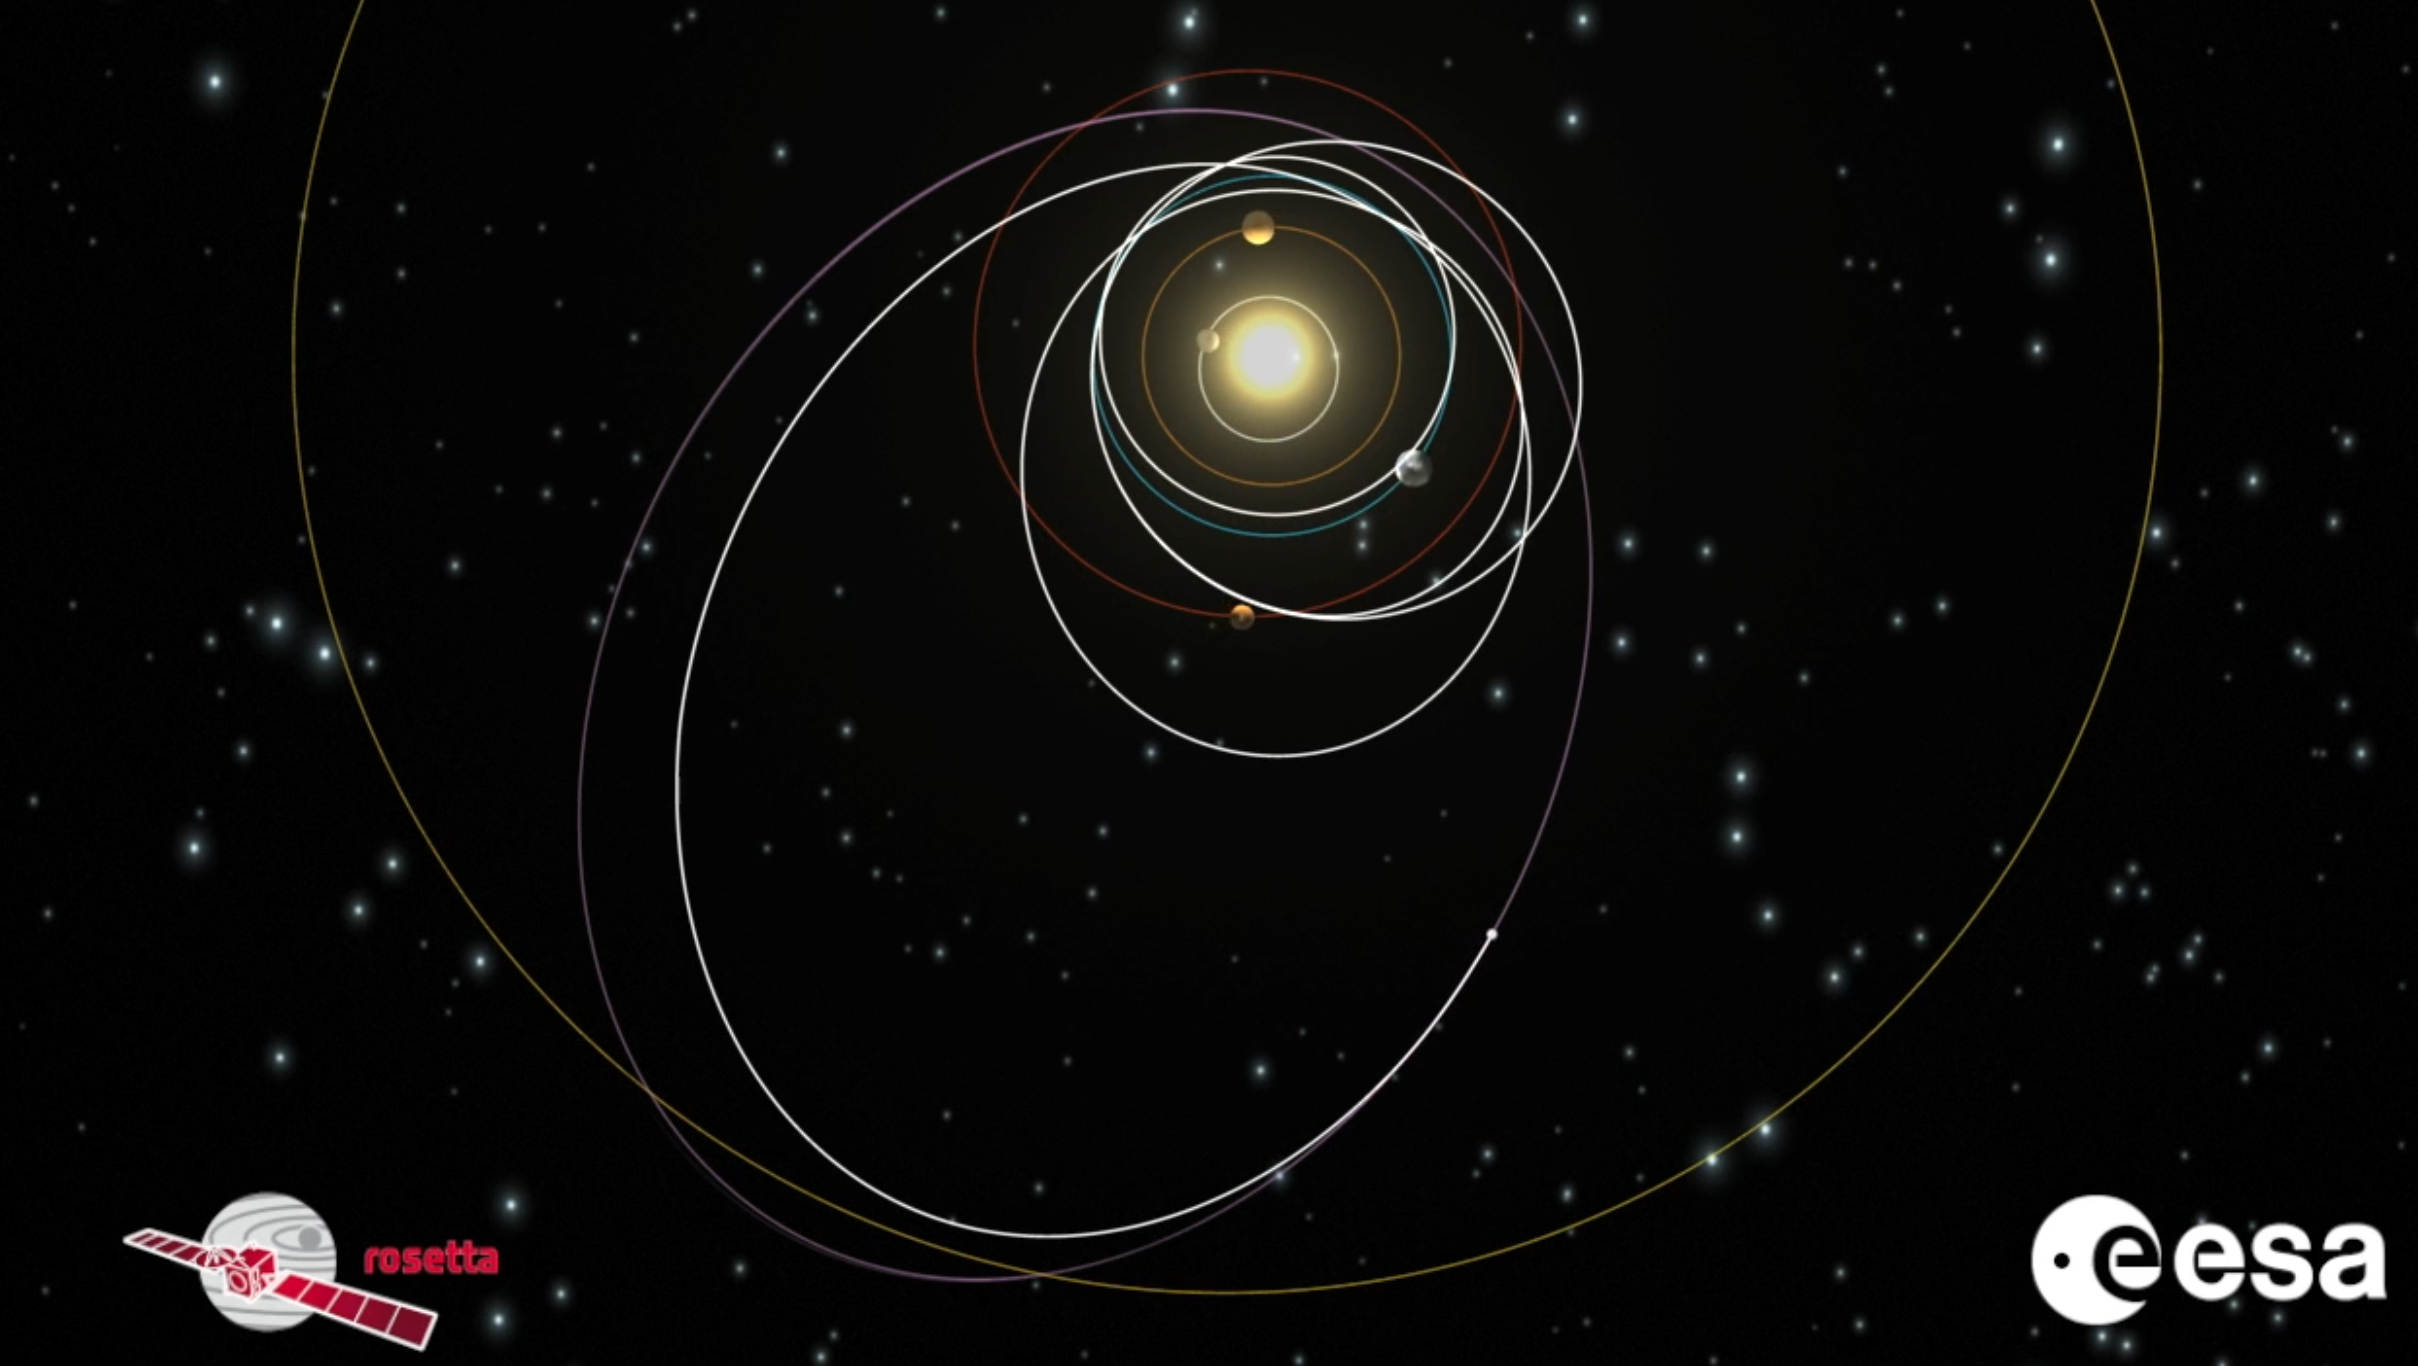
\includegraphics[height=.5\textheight]{./fig/rosetta.png}\\
Trajet de Rosetta pour atteindre  la comète 67P/Churyumov-Gerasimenko après 12 ans de voyage
\end{figure}
\end{frame}


\begin{frame}
\frametitle{Machine learning}
\begin{alertblock}{}
Les méthodes de machine-learning ont connu dernièrement un \alert{essor très important} à travers l'utilisation de nouveaux concepts (réseaux profonds) associés à du calcul haute-performance (notamment GPU).
\end{alertblock}
\begin{figure}
\begin{tikzpicture}
  \begin{axis}[title  = ILSVRC top error (by year),
    height = .55\textheight,
    width = .8\textwidth,
    ybar,
    x axis line style = { opacity = 0 },
    axis y line       = none,
    tickwidth         = 0pt,
    enlarge x limits  = 0.2,
    enlarge y limits  = 0.02,
  symbolic x coords = {2010, 2011, 2012, 2013,2014},
    nodes near coords,
  ]
  \addplot coordinates { (2010,28.2)    (2011,25.8) (2012,16.4) (2013,11.7) (2014,6.7)};
  %\addplot coordinates { (14320,LaTeX)         (1615,Tools)
  %                       (560,Distributions)   (3075,Editors)  };
  %\legend{Topics, Posts}
  \end{axis}
  \end{tikzpicture}\\
  ImageNet Large Scale Visual Recognition  Challenge\\
 \raggedleft {\footnotesize{\textit{from Russakovsky et al. 2014}}}
  \end{figure}
\end{frame}

\begin{frame}
\frametitle{Données et modélisation physique ?}
\begin{columns}

\column{.5\textwidth}
Beaucoup de données
\column{.5\textwidth}
Des modèles complexes
\begin{figure}
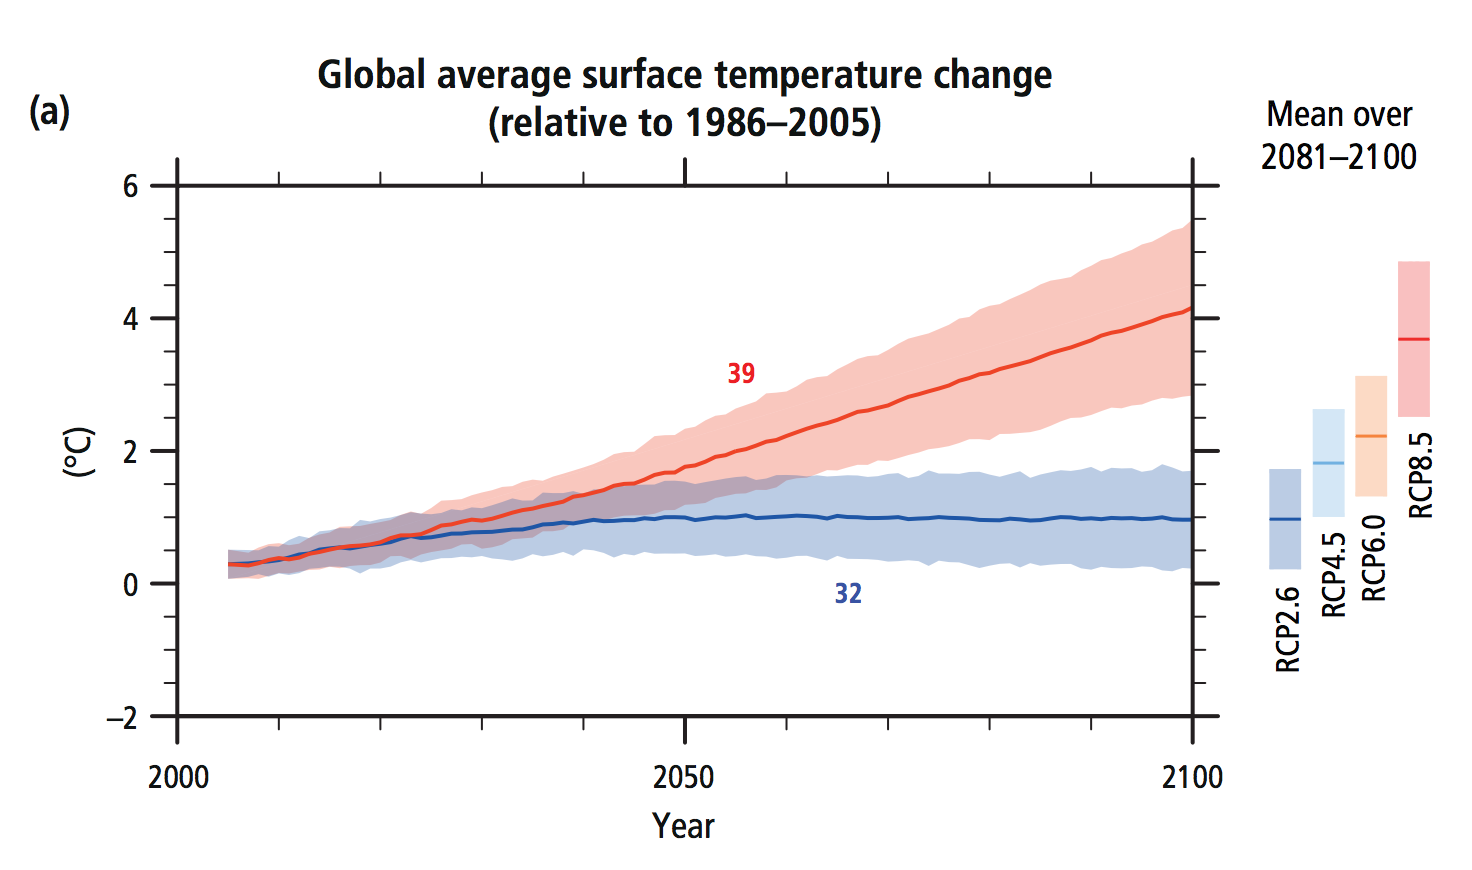
\includegraphics[width=\textwidth]{./fig/ipcc.png}\\
\raggedleft{\footnotesize{\textit{from IPCC Synthesis Report (2014)}}}
\end{figure}

\end{columns}
\end{frame}

\begin{frame}
\begin{figure}
\begin{tikzpicture}
  \begin{scope}[blend group = soft light]
    \fill[red!40!white]   ( 90:1) circle (2.5);
    \fill[green!40!white] (210:1) circle (2.5);
    \fill[blue!40!white]  (330:1) circle (2.5);
  \end{scope}
  \node at ( 90:2.7)    {Inria};
  \node at ( 210:2.7)   {LIP6};
  \node at ( 330:2.7)   {LOCEAN};
  \node [text centered, text width=80pt,font=\small] {\textbf{Probl\'ematique g\'eophysique}\\ (ex : Mer M\'editerran\'ee)};
  \node at (30:2.2) [text centered,text width = 40pt,font=\scriptsize, anchor=center] {Stage Inria-LOCEAN};
  \node at (150:2.2) [text centered,text width = 40pt,font=\scriptsize\scriptsize, anchor=center] {Stage Inria-LIP6};
  \node at (270:2.2) [text centered,text width = 40pt,font=\scriptsize, anchor=center] {Stage LIP6-LOCEAN};

\end{tikzpicture}
\end{figure}
\end{frame}
\end{document}
